% Chalmers title page
\begin{titlepage}

\AddToShipoutPicture{\backgroundpic{-4}{56.7}{include/images/frontpage}}
\mbox{}
\vfill
\addtolength{\voffset}{2cm}
\begin{flushleft}
\begin{figure}
    \centering
    \vspace{5mm}
    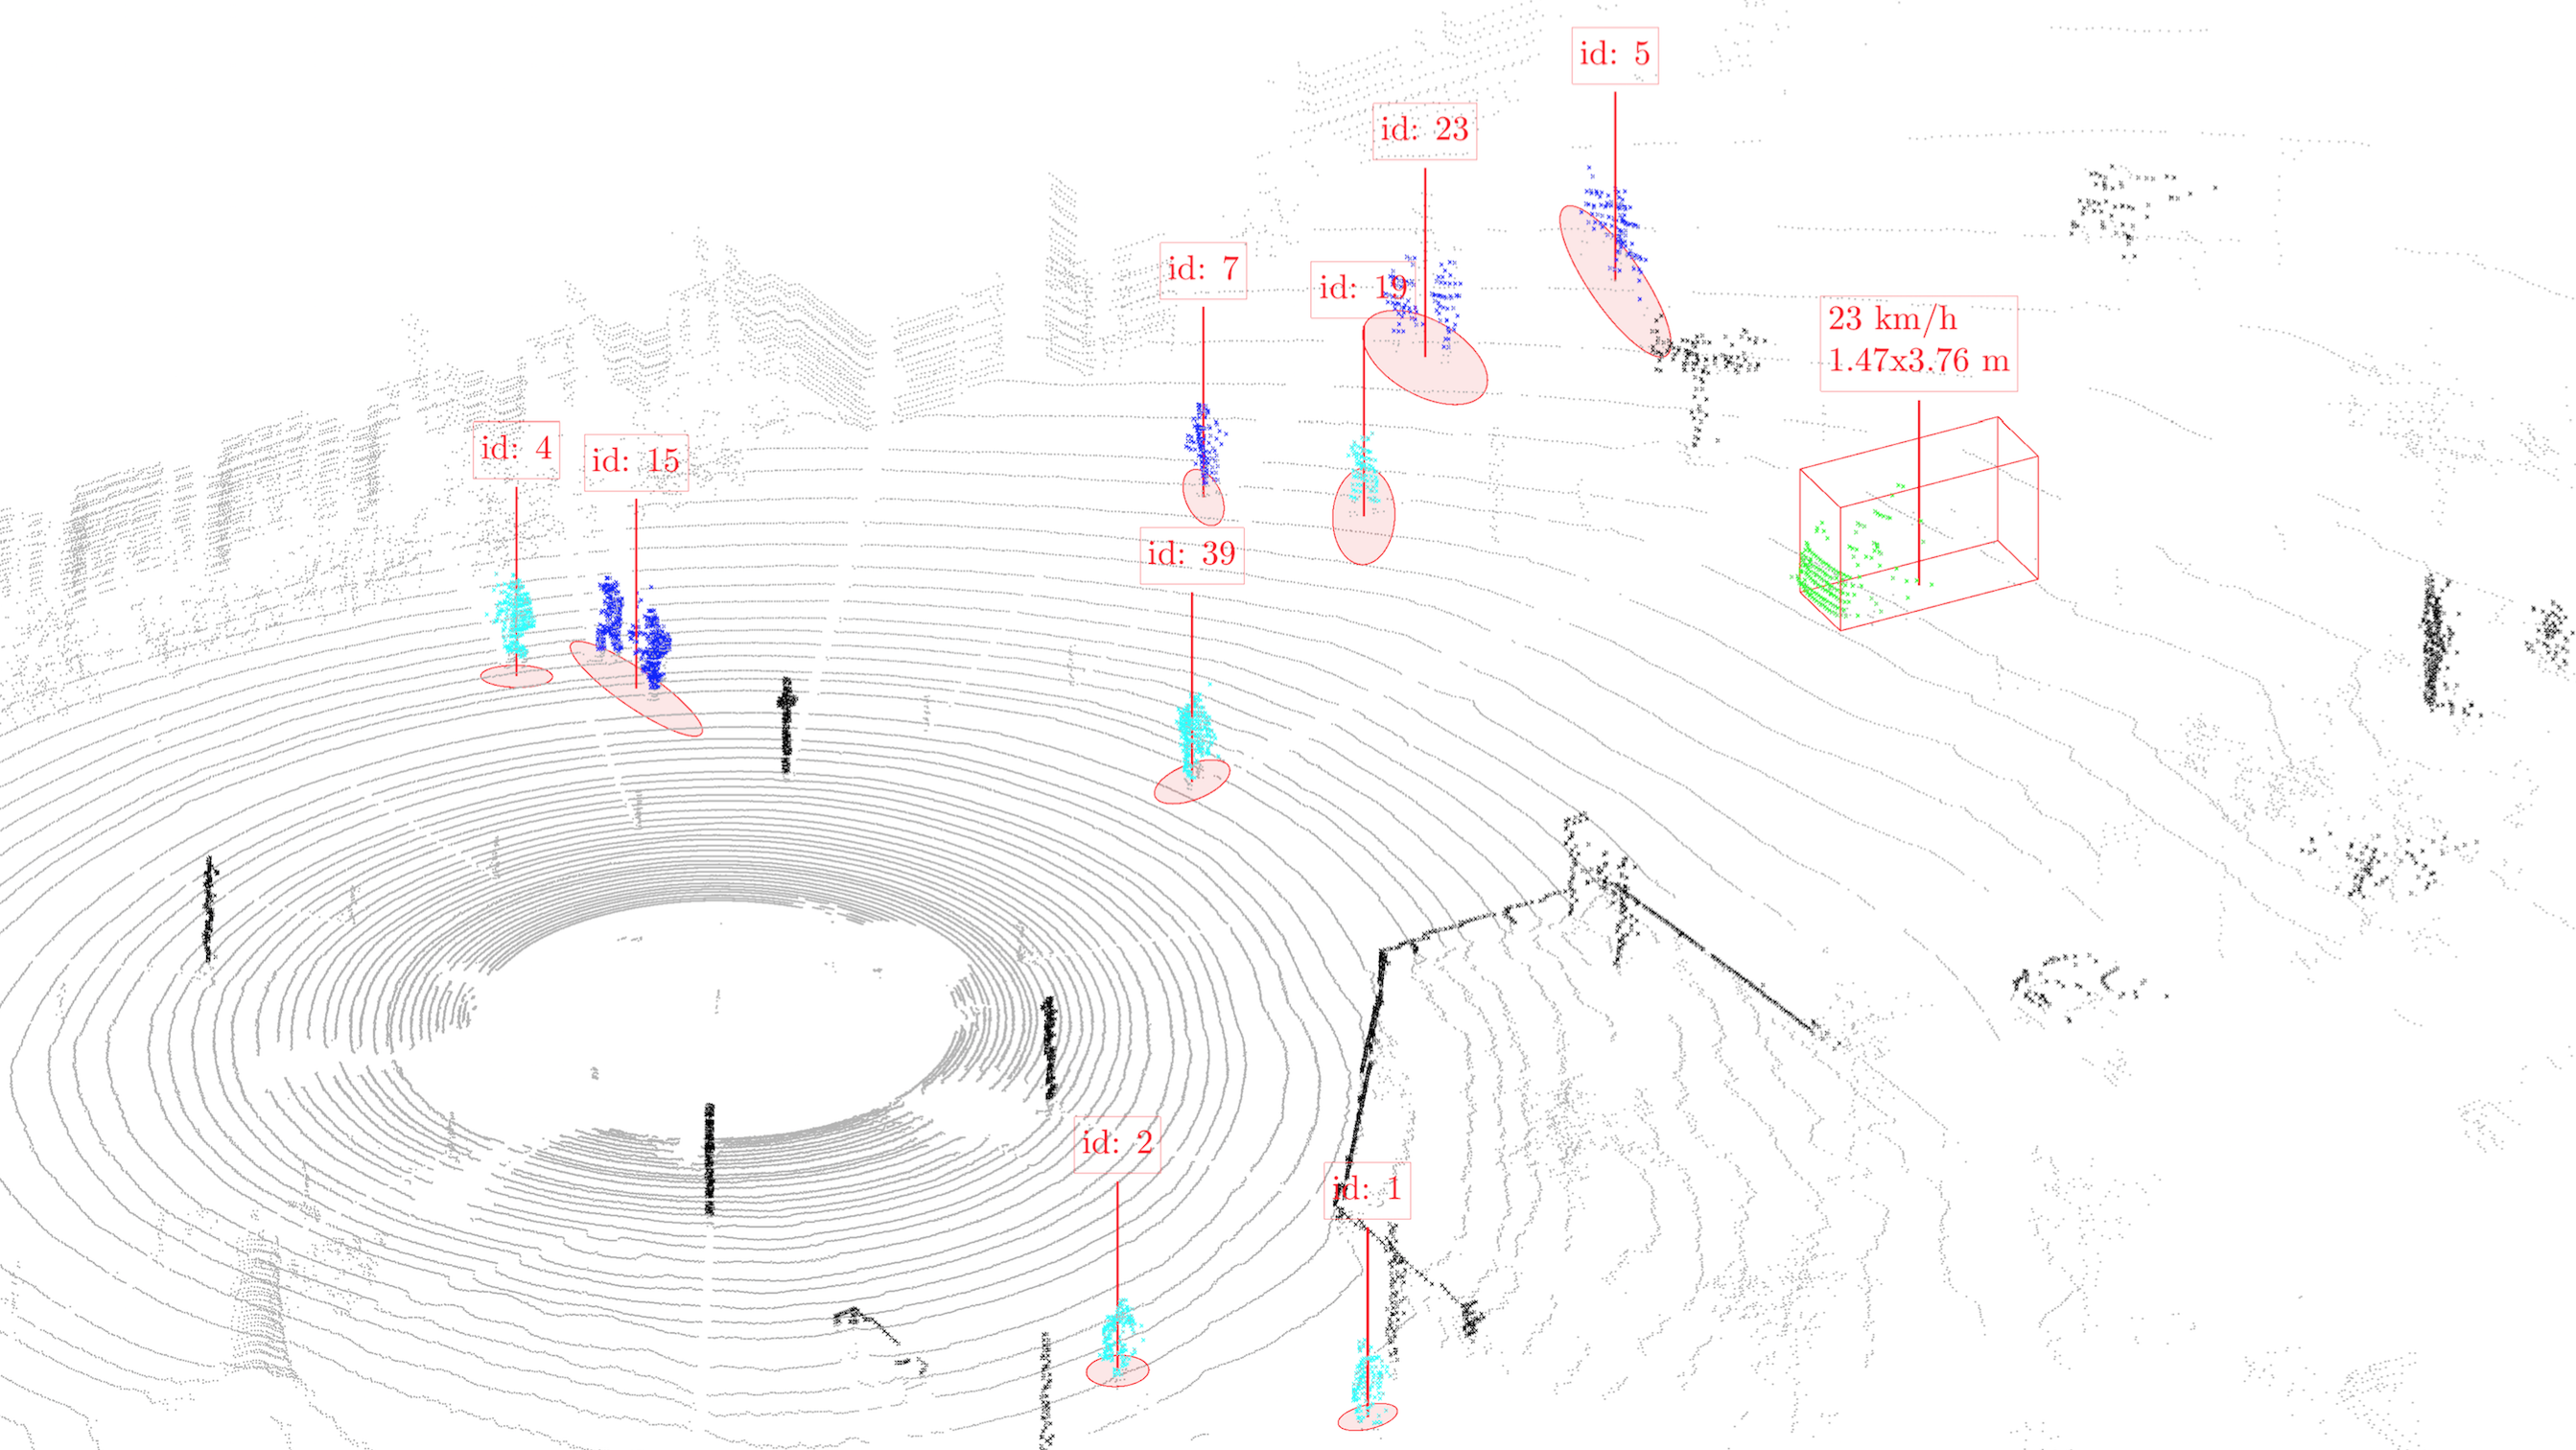
\includegraphics[width = 1\linewidth]{include/images/frontFin.png}
\end{figure}
	{\noindent {\Huge Lidar-based Methods for Tracking and Identification } \\[0.5cm]
	{\Large A NN-GIW-ETT-IMM-UKF-PHD filter} \\[0.5cm]
	\emph{\Large Master's Thesis in Systems, Control \& Mechatronics} \\[.8cm]
	
	{\huge Marko "Marky Mark" Cotra\\ Michael "The Snail" Leue}\\[.8cm]
	
	{\Large Department of Signals \& Systems \\
	\textsc{Chalmers University of Technology} \\
	Gothenburg, Sweden 2016 \\
	Master's Thesis 2016:1\\
	} 
	}
\end{flushleft}

\end{titlepage}
\ClearShipoutPicture
% End Chalmers title page

\pagestyle{empty}
\newpage
\clearpage
\mbox{}
\newpage
\clearpage
\thispagestyle{empty}

\begin{abstract}
Active safety systems and autonomous drive functionality are being developed as an increasingly important competitive advantage for car manufacturers. Modern cars are equipped with a variety of sensors such as radar, ultrasound, GPS or camera. All of those information streams are then fused into an optimal estimation of the surrounding environment in order to follow a certain trajectory or avoid collisions with other objects. In order to test accuracy of the aforementioned sensors, costly high precision GPS sensors are placed on objects of interest around the car. Therefore a more cost effective and easy to use system for sensor validation is desirable, preferably enabling real-time performance feedback.

A promising method for creating such a system is by utilizing high-resolution data created by a lidar sensor. State-of-the-art lidar sensors are capable of capturing very detailed information about the surroundings in the form of a point cloud with up to 150,000 points per scan. Not only can this data be used to verify other sensors, it also opens up a new level of tracking dynamic (non-stationary) objects around the vehicle. In addition to the kinematic state (position, velocity, acceleration) the highly structured point data can be used to estimate the shape and size of objects of interest very accurately. However, the sheer amount of data requires a quite sophisticated pre- processing pipeline that removes irrelevant parts and partitions the point cloud into clusters. As such, utilizing prior knowledge about the surrounding environment is of importance.

This thesis describes the implementation of a tracking algorithm to both estimate the kinematic state as well as shape and size of a time varying and unknown number of dynamic objects in lidar data. A prerequisite for the algorithm is available prior knowledge about the static surrounding environment. The algorithm is based on Bayesian inference. Methods and techniques normally used with other sensor types, such as radar and camera, are modified for usage with lidar data and used by the algorithm. Inferences on the shape of objects are modelled as either elliptical or rectangular, based on the type of target. In addition to that, a supervised neural network is trained to accurately classify detected objects (e.g. car, cyclist, pedestrian). This enables the algorithm to apply specific tracking approaches for the different kinds of targets and more effectively dismiss clutter measurements that are not deemed to be important.

The tracking algorithm is evaluated using real data with four defined categories of targets: pedestrian, car, bicycle and crowd. Rectangular shape estimation is used for cars and elliptical shape estimation for the remaining classes. Both tracking and identification of objects is achieved with high precision. However, due to a lack of reference system only visual evaluation of algorithm performance was made. Additionally, computational complexity is evaluated from a theoretical standpoint.

The algorithm proposed in this thesis indicates that lidar sensor data can be used to successfully identify and track dynamic objects of interest around a car. Testing the algorithm using data where high precision GPS systems are attached on all objects of interest is needed in order to determine how suitable of a replacement a lidar based system would be. Additionally, an implementation of the algorithm on an embedded system should be performed in order to evaluate potential real-time use. 

\end{abstract}

\newpage
\clearpage
\mbox{}
\newpage
\clearpage
\thispagestyle{empty}
\section*{Acknowledgements}
Mention Karl's and Lennart's help here?\todo{marko's acknowledgements}

Marko would like to thank his friends and family for all their support. He would especially like to thank his father Nenad Cotra for inspiring him to become an engineer. 

He also wants to acknowledge Steve Jobs for inventing the computer, as well as Bill Gates for inventing the Internet and Chrome. Without them, none of this would have been possible.

Michael would like to thank his parents Hartmut and Kathrin Leue for their continuous support throughout his life. He would not be where he is without them, not even close. \textit{Danke für alles.}

He also wants to express his sincere gratitude towards the many free and open pieces of software that were used to realize this thesis, mainly Ubuntu GNU/Linux with the GNU base system and the Gnome software suite, Firefox, Vim, Octave and \LaTeX. Thanks to all the helpful souls out there that make those tools available to everyone, free of charge.
\\[1cm]

\hfill Marko Cotra \& Michael Leue, Gothenburg, June 2016 
\newpage
\clearpage
\mbox{}